\chapter{Methods} \label{chap:methods}
\section{Idea Generation} 
The idea generation followed a ''divergent - emergent - convergent'' process~\cite{gameBook}, as seen in Figure~\ref{fig:ideaGeneration}. At the first stage, we conducted a brainstorming session, where each group member freely expressed their ideas related to VR and AR in the field of games, health or education. A range of ideas was generated, including a rehearsal room for musicians or dancing classes, a public speaking practice place, collaborative painting or sand painting, a virtual memory palace, a 3D-data visualisation room and simulators for activities like gardening, parachuting or car racing. 

After discussing all ideas we decided to apply dot-voting~\cite{gameBook} which helped us to prioritize our favourite ideas. All of us received three votes and we were able to allocate the votes (dots) as we saw fit. This meant that we could put all three dots on one of the ideas or we could put one dot on three different ideas instead. When everyone had placed all their dots, we narrowed our focus to the three ideas with the most votes. 

One of the ideas was to create a service which lets the musicians or DJs play their own music and artists to display visualisations, while an audience could meet in virtual space to experience the audio-visual performance and dance together. Another was an educational chemistry game, aimed at school children, and the final idea being an orchestral conducting game.

\begin{figure}[tbph]
    \centering
    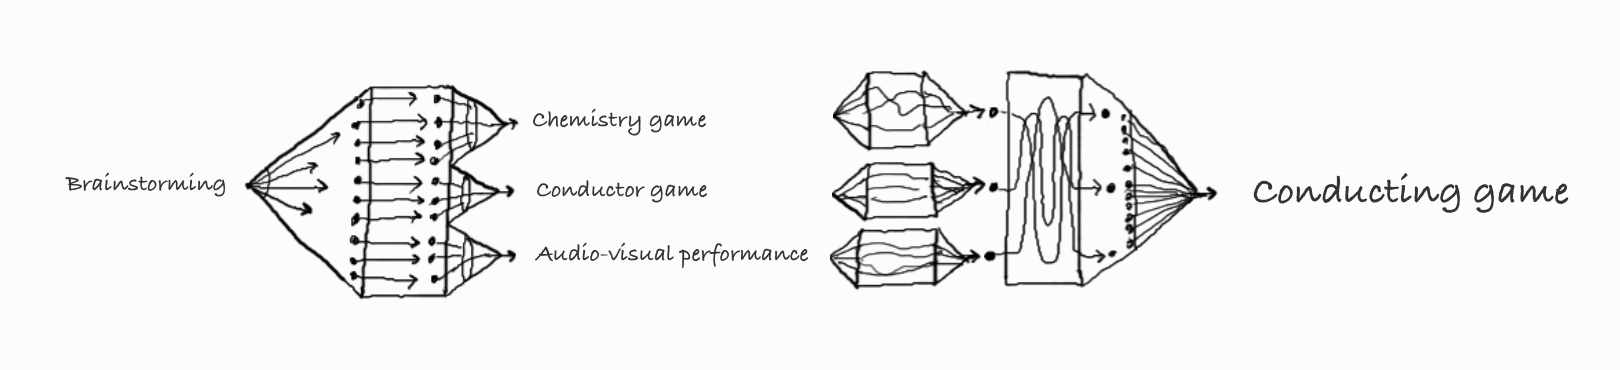
\includegraphics[width=1.0\textwidth]{images/ideaGenerationProcess.png}
    \caption[Idea Generation Process]{The process of idea generation~\cite{gameBook}}
    \label{fig:ideaGeneration}
\end{figure}

In the following discussion of these ideas, we sketched the scenarios of the games, as well as the implementation details. We now had a better feel for, and understanding of, each idea. Together we decided that we would like to try to develop the orchestra conductor game. Among the reasons for this choice was the strong musical background of four group members, as we believed our musical experience would help us to create a more interesting game scenario. The lack of market competitors also played a part in our decision, additionally, the VR technology seemed to suit conducting well. Sketching of ideas was further used in the project to illustrate our ideas to each other as seen in Figure~\ref{fig:tablesketch} which contains a sketch for how we envisioned the various elements of the Conductor Table. 

\begin{figure}[tbph]
    \centering
    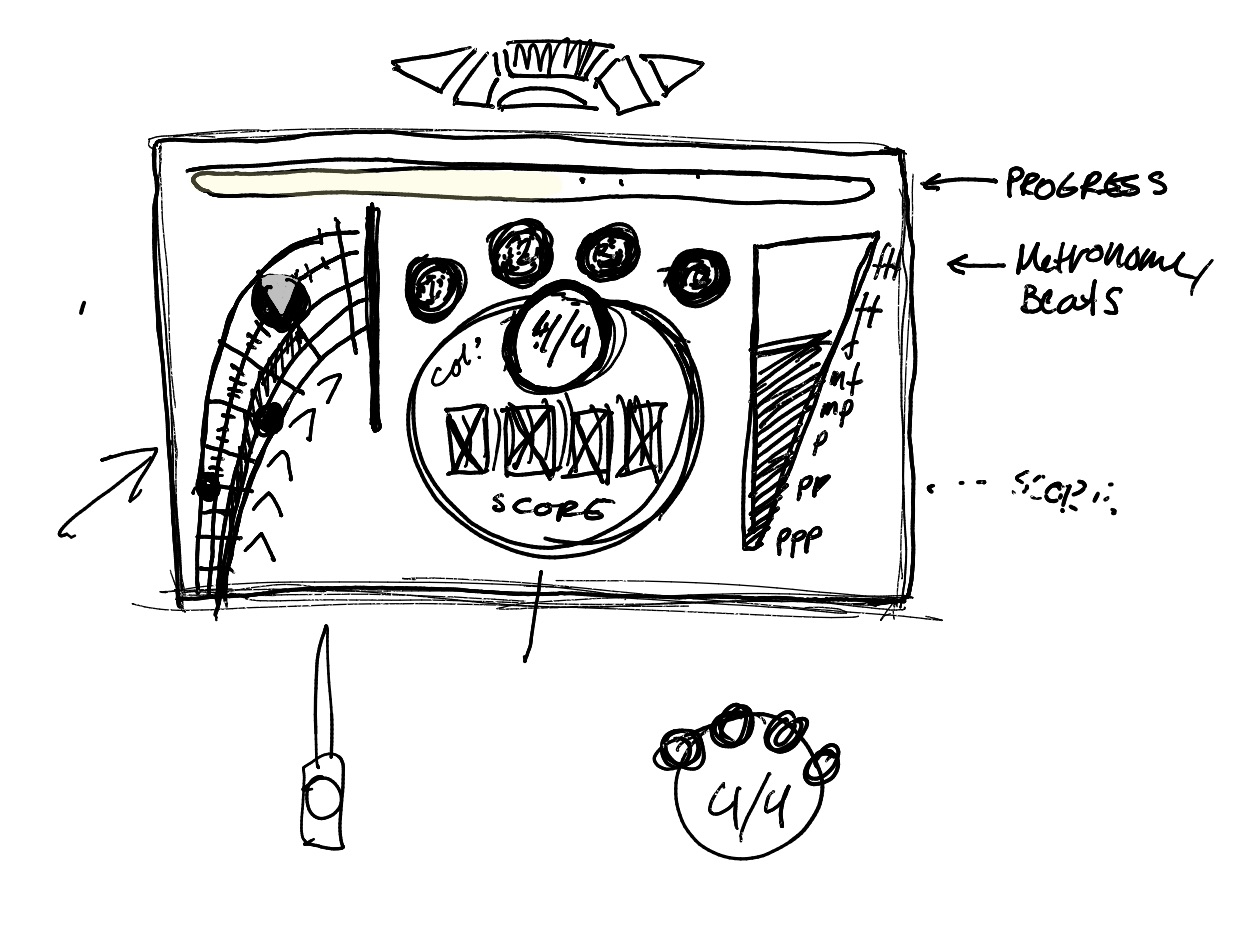
\includegraphics[width=0.75\textwidth]{images/sketch.jpg}
    \caption[Example sketch of the Conductor Table]{This Figure contains a sketch for how the Conductor Table initially was supposed to look like.}
    \label{fig:tablesketch}
\end{figure}

\section{Interview}
After choosing to develop a conducting game, we interviewed a professional conductor over Skype to learn more about his experience of conducting and conductor training. The purpose of the interview was to better understand the different aspects of conducting. We also wanted to explore possibilities of involving VR games to promote the positive sides of conducting and to make any negative sides of the training process seem more engaging. During the interview, we found one motivation for the role of conducting, which is the feeling of control and leadership, as the orchestra follows your directions. It is relatively hard to get access to a whole orchestra for conducting training in real life, especially for conducting fanciers or novices. However, in a VR environment, it is possible to have access to a virtual orchestra with a customized composition at any time as long as the player has access to a VR device. With the interactions and feedback from the virtual orchestra, players can achieve greater motivation to keep on training. From the interview, we also got the idea that using unique virtual environments and game elements may ease the feeling of dullness and stress during repeated training. The feedback from the conducting expert confirmed pre-existing assumptions for the features in the conductor game and helped us to have a clearer vision about potential users.

\section{Tools}
The game was created using the Unity engine (version 2017.3.0.3f) with C\# as a language for the scripting components. Microsoft's Visual Studio 2017 Community was used as the Integrated Development Environment. Version control was done through Git using Github as our hosting service. Google drive was used for storing sound files, as these often came close exceeding Github’s restrictions on file size, and to a large extent slowed the system down.
Valve’s Unity SteamVR plugin was used for communicating with the HTC Vive. Blender was used for modeling 3D assets, like the instruments and game world. The UI for the conducting table was created with Adobe Illustrator and Adobe Photoshop. The soundtrack used for the game was composed in Guitar Pro 5. Cubase 5 was used as the Digital Audio Workstation when generating audio from the midi tracks exported from Guitar Pro 5, using Virtual Studio Technology instruments from EastWest/Quantum Leap symphonic orchestra to produce the desired individual instrument tracks. Discord was used for intragroup communication.


\section{Development Methodologies}
The development followed a mixed methodology model with a focus on aspects that would allow us to work in parallel and quickly prototype features. Code hygiene factors was a low priority due to the limited time and we did not expect that performance would be an issue with such a limited game. We, therefore, adopted a ''critical path coding''~\cite{critical_path_coding} approach to get as much done with as little code as possible.

Developers usually worked individually after short discussions on architecture, however, pair programming techniques were employed for more challenging or unfamiliar problems. 
We originally intended to have a focus on the process, making proper use of issue tracking, branching strategies, and code reviews. However, early in the project, we came to the conclusion that this added unnecessary overhead to a time-limited project. We decided it would be more beneficial for the project that we spent more time on implementation rather than documentation and process.

In terms of meetings, we employed daily three minute meetings during the morning of every village day in a similar vein to those used in agile software methodologies. These meetings consisted of every group member mentioning any additional progress that had happened since the last day, what they planned to work on during the village day and discussing any potential problems that may arise. We kept these meetings to a maximum of three minutes per group member as a means to avoid situations where certain group members could end up dominating the discussions.